\documentclass[twocolumn]{article}
\usepackage{graphicx}
\usepackage{amsmath}
\usepackage{float}
\usepackage{amssymb} %Use of therefore symbol
\usepackage{hyperref}
\usepackage{caption}



\begin{document}
\title{Lab 1: Monte Carlo Methods}
\author{Alex Matheson, Austin Nhung}
%\affiliation{Department of Physics and Astronomy, University of Calgary, Calgary AB T2N 1N4 Canada}
\date{\today}
\maketitle

\section{Introduction}
The Fourier transform is one of the mathematical marvels of the modern world. While it was invented in the early 19th century, it was instrumental in the communication's revolution beginning with radio, and continuing into the modern digital world. The Fourier transform is an extension of the fourier series, which expresses a function in terms of a basis of sinusoids or exponentials. The Fourier transform allows one to work on a problem either in its original space or in that of a Fourier space. There are many pairs of variables that may be connected by Fourier transform including time/frequency and position/wavenumber. By working in Fourier space, certain periodic patterns may be emphasized or de-emphasized in data. This is the basis of modern signal processing and filtering to remove noise. Fourier techniques have myriad applications outside the mathematical context of this assignment including audio-processing, radio-astronomy, and medical imaging.

\section{Methods}
\subsection{Fourier Series}
Fourier series are defined by calculating the Fourier coefficients $a_n$ and
$b_n$. These coefficients may be replaced with a complex Fourier series using
a single complex coefficient $c_n$. These coefficients are related through the
equations:
\begin{equation}
	\begin{split}
		a_n =& c_n + c_{-n} \\
		b_n =& i(c_n - c_{-n}) \\
		c_n =& \frac{1}{2}(a_n - ib_n)
	\end{split}
\end{equation}
In Fourier series, $a_n$ and $b_n$ correspond to even and odd 'components' of
the function, respectively. In the case of an even function, their relations
simplify to:
\begin{equation}
	\begin{split}
		a_n =& c_n + c_{-n} \\
		b_n =& 0 \\
		c_n =& \frac{1}{2}(a_n)
	\end{split}
\end{equation}

Meanwhile, odd functions simplfiy to:
\begin{equation}
	\begin{split}
		a_n =& 0 \\
		b_n =& i(c_n - c_{-n}) \\
		c_n =& \frac{-ib_n}{2}
	\end{split}
\end{equation} 

It can be shown in both of the above series that the $a_n$ term for even
functions and $b_n$ for odd functions will be proportional to the $c_n$ terms.
The complex coefficients are alternatively defined as:
\begin{equation}
	c_n = \frac{1}{2 \pi} \int_{-\pi}^{+\pi} f(x) e^{-inx} dx
\end{equation}
It is easy to see that $c_{-n} = c_n^{\ast}$, where $c_n^{\ast}$ is the complex
conjugate of $c_n$. The relation of squares can then be expressed:
\begin{equation}
	\begin{aligned}
		\sum_{n = -\infty}^{+\infty} \left| c_n \right|^2
		&= \sum_{n = -\infty}^{+\infty} \left| \frac{1}{2} (a_n - ib_n) \right|^2 \\
		&= \frac{1}{4} \sum_{n = -\infty}^{+\infty} \left(
		\left| a_n \right| + \left| b_n \right|^2
		\right)
		&= \frac{1}{2} \sum_{n=0}^{\infty} \left(
		\left| a_n \right|^2 + \left| b_n \right|^2
		\right)
	\end{aligned}
\end{equation}
Using the definition of $b_n$, this result can be further simplified knowing
that $b_0 = i(c_0 - c_0) = 0$ to reach the final form
\begin{equation}
	\sum_{n = -\infty}^{+\infty} \left\| c_n \right\|^2
	= \left\| \frac{a_0}{2} \right\|^2 + \frac{1}{2} \sum_{n=0}^{\infty} \left(
	\left| a_n \right|^2 + \left| b_n \right|^2
	\right)
\end{equation}

%Parseval's theorem relates the Fourier coefficients of a function to its power spectrum. Using the above relations, it may be restated in terms of sine and cosine coefficients, as shown below.

%\begin{equation}
%\begin{split}
%\int_{-\infty}^{\infty} |x(t)|^2 dt =& \sum_{n=-\infty}^{\infty} |c_n|^2 \\
%\sum_{-\infty}^{\infty} |c_n|^2 =& \sum_{n=-\infty}^{\infty} |\frac{1}{2}(a_n - ib_n)|^2 \\
%=& \frac{1}{2^2}\sum_{n=-\infty}^{\infty} (a_n - ib_n)(a_n + ib_n) \\
%=& \frac{1}{2^2}\sum_{n=-\infty}^{\infty} |a_n|^2 + |b_n|^2 \\
%=& \frac{1}{2^2}\sum_{n=0}^{\infty} |a_n|^2 + |b_n|^2 \\
%=& \frac{|a_0|^2}{2^2} + \frac{1}{2^2}\sum_{n=1}^{\infty} |a_n|^2 + |b_n|^2 \\
%\end{split}
%\end{equation}

Next, a square wave function was considered as defined below: 

\[ 
f(t)=
\begin{cases}
1, & |t| \leq T/4 \label{eq:square}
\\
0, & |t| > T/4
\end{cases}
\]

\begin{figure}
\centering
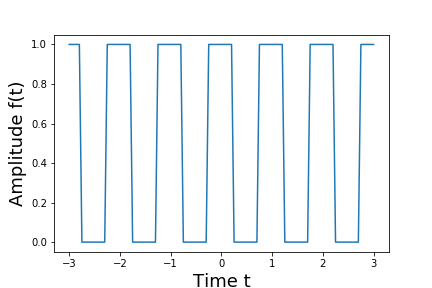
\includegraphics[width=\linewidth]{Figure1}
\caption{Piecewise function defined in equation \ref{eq:square}. The function is a form of a traditional square wave.}
\label{fig:Figure1}
\end{figure}


This function was periodic between $-T/2$ and $T/2$. The function was visualized in figure \ref{fig:Figure1}. As with any function, this could be re-stated using complex Fourier series. To compute the series, the coefficients $c_n$ were determined according to equation \ref{eq:complex_coefficients}. 

\begin{equation}
c_n = \frac{1}{T} \int_{-T/2}^{T/2} f(t) \exp(-i\frac{2\pi nt}{T}) dt
\label{eq:complex_coefficients}
\end{equation}

The coefficients could be solved analytically, yielding the answer $c_n = \frac{-i}{\pi n}$ for $n = 1, 3, 5, ...$. As the found $n$ values suggest, the original function was purely odd, meaning that the function could be constructed from purely sine terms. Due to this, all even $c_n$ terms (including $c_0$) are $0$. The values of the different $c_n$ terms may also be plotted, as shown in figure \ref{fig:Figure2}. The values in this plot show that the odd $n$ terms follow a hyperbolic sinusoid path. The complete series may be written as:

\[
f(t) = \sum_{n= -\infty}^{\infty} -\frac{i}{\pi n} \exp(-i \frac{2\pi nt}{T})
\]

\begin{figure}
\centering
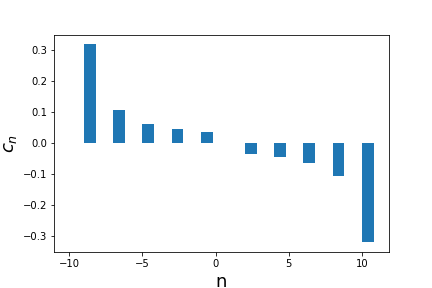
\includegraphics[width=\linewidth]{Figure2}
\caption{Values of each term $c_n$ in the complex fourier series.}
\label{fig:Figure2}
\end{figure}

The Nyquist frequency defines the upper limit of frequency detectable by a given sample rate. This principle also works in reverse. Since the human ear can hear frequencies up to 20 kHz, a sampling inteval would need to be less than 25 $\mu s$ for a sampling rate of 40 kHz.

\subsection{FFT}
Four simple analog signals were used to analyze the behaviour and consequences
of sampling a signal and using the discrete Fourier transform. The signals used
were:
\begin{equation}
	\begin{aligned}
		f_1(t)  &= \sin(2 \pi \times 100 t) + \frac{1}{2} \sin(2 \pi \times 200 t) \\
		f_2(t) &= \sin(2 \pi \times 100.5 t) + \frac{1}{2} \sin(2 \pi \times 200 t) \\
		f_3(t) &= \left( 2 + \sin(2 \pi \times 8 t) \right) \times \sin(2 \pi \times 100 t) \\
		f_4(t) &= \sin \left( 2 \pi \times 100 \left( 1 + \frac{1}{10} \sin(2 \pi \times 8 t) \right) t \right)
	\end{aligned}
	\label{fft_eqs}
\end{equation}

These signals were sampled at a rate of $1024$ samples per second for one second
each. They were then transformed into the frequency domain using the fast
Fourier transform (FFT). The amplitudes and power spectra are shown in figure \ref{fig:fft_exs}.

\begin{figure*}
	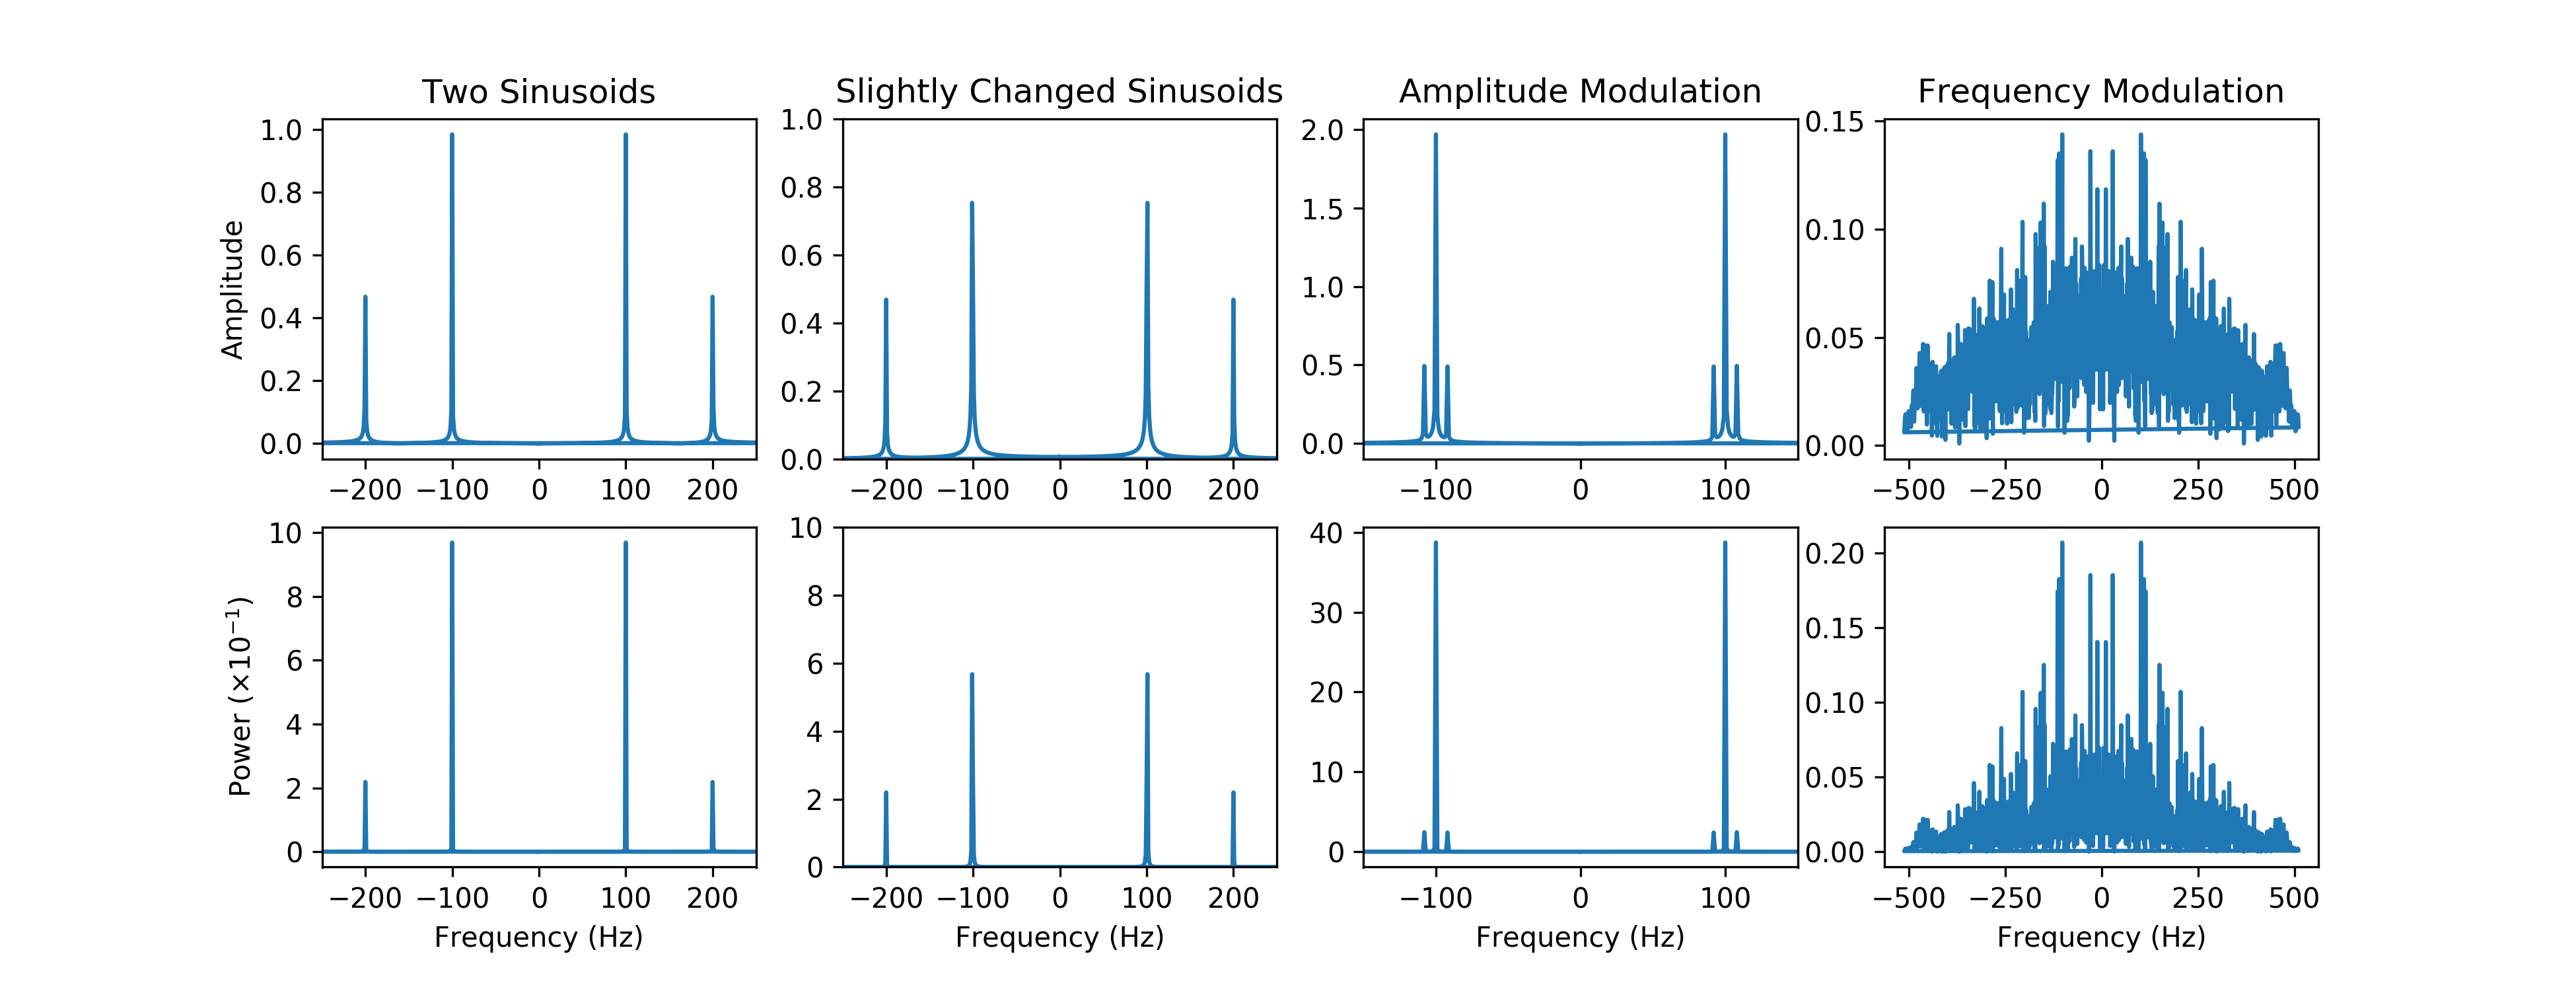
\includegraphics[width=\linewidth]{fft_examples.png}
	\caption{
		The amplitude (top row) and corresponding power (bottom row) spectra of the
		signals described in \ref{fft_eqs} in the same order from left to right.
	}
	\label{fig:fft_exs}
\end{figure*}

The first signal is simply the sum of two sines at frequencies $100$Hz and
$200$Hz with amplitudes $1$ and $0.5$, respectively. This is evident on the
two leftmost panels in figure \ref{fig:fft_exs}. The second signal is only
slightly different from the first, yet the amplitude and width of the peak at
$100$Hz is noticably different. This is because the number of samples limits the
number of bins that will be calculated and the sampling frequency limits the
highest frequency. Since the sampling rate is $1024$Hz and there are $1024$
samples, each frequency bin is $2$Hz. $100$Hz was easily resolved since it is a
multiple of $2$, but this is also the reason why $100.5$Hz was not.

The other signals are examples of amplitude and frequency modulation. The
amplitude modulated signal involves multiplying sines together, which can be
expressed as:
\begin{equation}
	\sin(\alpha) \times \sin(\beta) = \frac{1}{2} \left(
	\cos(\alpha - \beta) - \cos(\alpha + \beta)
	\right)
\end{equation}
This is the resulting signal in the third column of figure \ref{fig:fft_exs}
where the peaks occur at $100$Hz as well as $100 \pm 8$Hz. Frequency
modulation can be thought of as varying the frequency of the signal over time.
This is the reason that its Fourier transform is spread across the entire range
of frequencies.

\subsection{Noise}
\subsubsection{Autocorrelation and PSD}
The autocorrelation function was examined in a previous lab. It turns out that the auto-correlation function may be applied to random signals (i.e. noise) as well. For white noise created from a uniform distribution of frequencies, the autocorrelation function is expected to be a delta function. Consider an ideal random number generator separate from the realities of computing. By definition, a number correlates with itself completely, forming a spike at $k=0$. For ideal noise, there is no relation between the first number generated, and any subsequent number generated. This means that subsequent values should yield $k=0$. Taken together, this is a description of $\delta(k)$.

The power spectral density function is connected to the auto-correlation function by the following formula:

\[ S(\omega) = \sum_{-\infty}^{\infty} AC(k)e^{-j\omega k} \]

Using this, the PSD of white noise may be calculated:

\begin{equation}
\begin{split}
S(\omega) =&  \sum_{i=-\infty}^{\infty} \delta (k) e^{-j\omega k}\\
S(\omega) =& \delta(k=0) e^{-j\omega * 0} \\
S(\omega) =& 1
\end{split}
\end{equation}

The above mathematical relations were tested using uniform random numbers on the interval $[0,1)$. For $8192$ numbers, the auto-correlation and associated power spectral density were plotted in figures \ref{fig:uniformAC} and \ref{fig:uniformS}. In order for these plots to behave as expected, the algorithm for auto-correlation provided in lab 1 required modification. The original algorithm for each $k$ summed over terms $1\to N-k$. This meant that higher $k$ values were subject to wide fluctuations due to deceasing denominator terms. By writing the algorithm to consider all other random numbers except the 'kth' random number in sums, the results were as expected. The power spectral density fluxuated, but had a mean of $0.969$ near the expected $S(\omega)=1$.

\begin{figure}
\centering
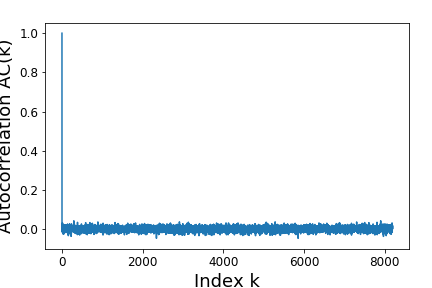
\includegraphics[width=\linewidth]{uniformAC}
\caption{Autocorrelation function from uniform numbers generated using numpy's random.rand() function.}
\label{fig:uniformAC}
\end{figure}

\begin{figure}
\centering
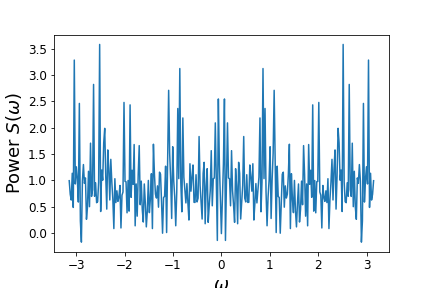
\includegraphics[width=\linewidth]{uniformS}
\caption{Power spectrum density of white noise created from uniform random numbers. The auto-correlation values in figure \ref{fig:uniformAC} were used to calculate the PSD.}
\label{fig:uniformS}
\end{figure}

Calculation of the auto-correlation function and PSD was repeated for white noise generated by a Gaussian distribution. Figures \ref{fig:GaussianAC} and \ref{fig:GaussianS} show the results obtained. The PSD had a mean value of $1.07$.

\begin{figure}[t]
\centering
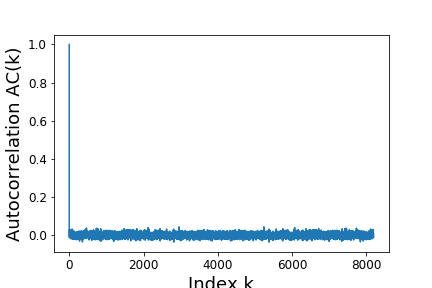
\includegraphics[width=\linewidth]{GaussianAC}
\caption{Autocorrelation function of white noise generated by random Gaussian numbers.}
\label{fig:GaussianAC}
\end{figure}

\begin{figure}
\centering
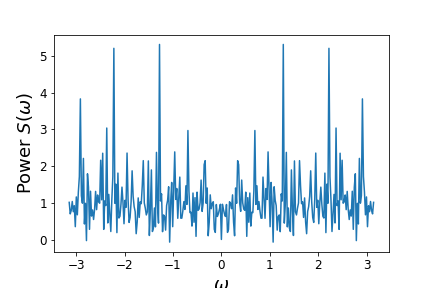
\includegraphics[width=\linewidth]{GaussianS}
\caption{Power spectral density of random white noise generated from a Gaussian distribution. This plot was created using autocorrelation data from figure \ref{fig:GaussianAC}.}
\label{fig:GaussianS}
\end{figure}


\subsection{Spectral Subtraction}
The spectral subtraction method involved Fourier transforming a signal, and then setting frequency bin values to zero if they were below a certain threshold. A signal was created using the formula $ x(t) = \sin (2\pi f_0t) + 0.5\sin (2\pi (2f_0)t)$ using $f_0=440$ Hz sampled at $22.2\mu s$, for $512$ intervals. Figure\ref{fig:spectral_filter}a shows this signal. The power spectrum of the signal was found using numpy's FFT package. Figure \ref{fig:spectral_filter}b shows this corresponding power spectrum. Two clear peaks were visible at $0.00976$ and $0.01953$. This matches almost exactly the expected values of $0.9768$ and $0.19536$ obtained by multiplying the frequency by the sampling period.

To investigate the impact of noise on the signal, random noise on the order $\pm 0.5$ was added to the signal. Figures \ref{fig:spectral_filter}c and \ref{fig:spectral_filter}d show the noisy power spectrum. The noise in this power spectrum was almost imperceptible compared to the signal in the neighborhood of the expected peaks. By outputting the power data, it was seen that the noise was on the order of $10^{-1}$. Some noise was slightly beyond one order of magnitude above or below this, indicating that the noise was not 'ideal' white noise.

Next, the threshold at which the magnitude of the noise cause the underlying signal to be totally obscured was determined. This was done by steadily increasing the noise magnitude until the signal peaks were on the order of the peaks from noise. Figure \ref{fig:spectral_filter}e and \ref{fig:spectral_filter}f show the corresponding signal and power spectrum.


\begin{figure*}[pt!]
	\centering
	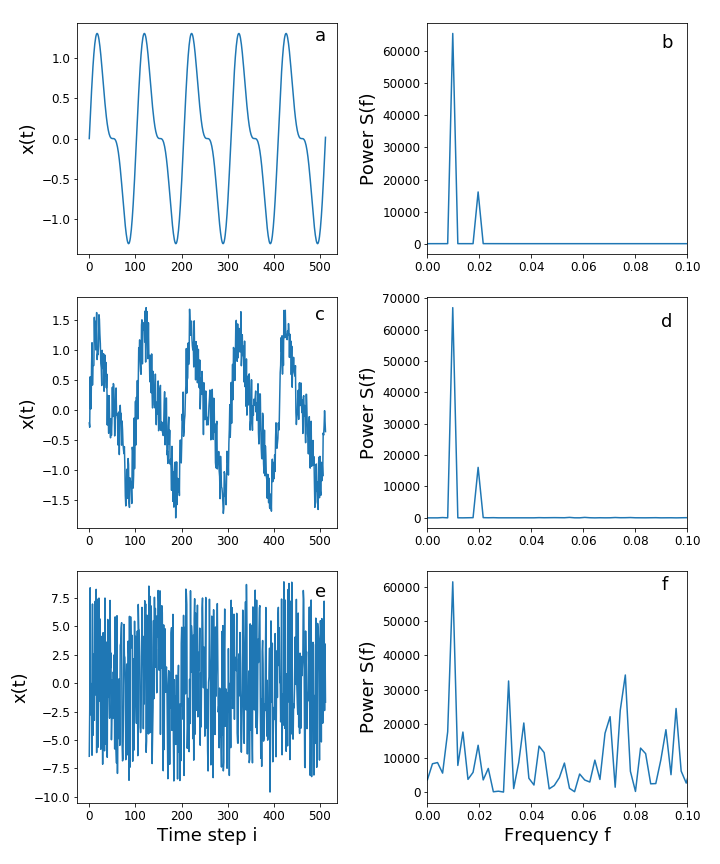
\includegraphics[height=\paperwidth]{spectral_filter}
	\caption{Effects of uniformly distributed (in time space) noise on a signal. Subplot \textbf{a} shows the original input signal, subplot \textbf{c} a signal with noise of $\pm0.5$ from the original signal, and subplot \textbf{e} the signal with $\pm10$ noise. The subplots immediately to the right are the corresponding frequency power spectra.}
	\label{fig:spectral_filter}
\end{figure*}

\subsubsection{Signals with Trends}
In this section, a periodic signal was laid over a linear trend to produce a new function. The original periodic function was $x_i = 2\sin(\pi f_0 i) + \cos( \pi f_1 i)$ while the trend function was $g(i) = 1 + 0.025i$ (constants of $f_0 = 9/512$ and $f_1=4/512$ were used). When added together, the two functions produced a new function, visualized in figure \ref{fig:trend}.

Next, the signal was made noisy using uniform noise of $\pm6$ added to the function. Figure \ref{fig:trendy} shows the result. The shape is largely still visible, only appearing "fuzzier".

\begin{figure}[t]
\centering
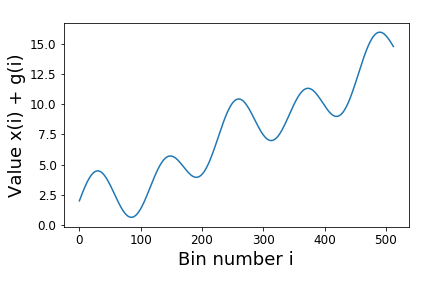
\includegraphics[width=\linewidth]{trend}
\caption{Function obtained by adding together a periodic and a linear function.}
\label{fig:trend}
\end{figure}

\begin{figure}
\centering
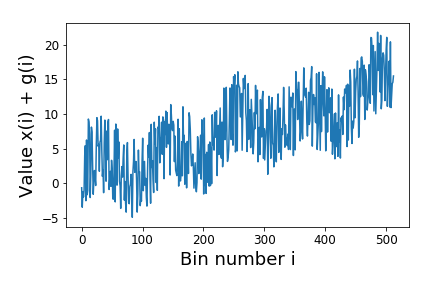
\includegraphics[width=\linewidth]{noise_trend}
\caption{Function from figure \ref{fig:trend} with uniform noise applied.}
\label{fig:trendy}
\end{figure}

As earlier in this lab, the FFT was used to examine the data for the underlying periodicity. Figure \ref{fig:trend_fft} showed the resulting power spectrum. The data was confined to a single, massive spike at $f=0$. For a noisy signal, the noise would be expected to manifest as a uniform addition across the power spectrum. This would still allow the original frequencies to be recovered. The lack of any distinct periodic peaks (the $f=0$ peak corresponds to non-periodic components) suggests that the linear component has erased the ability to check periodicity in the power spectrum. 

\begin{figure}
\centering
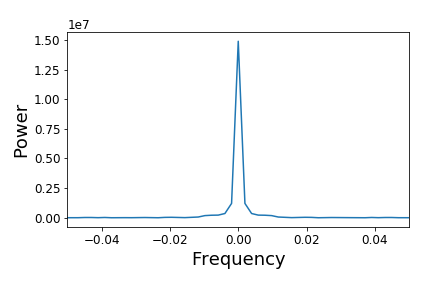
\includegraphics[width=\linewidth]{trend_fft}
\caption{FFT of the noisy function in figure \ref{fig:noise_trend}. The result was focused on the region near $f=0$ to ensure that there were not peaks close to $f=0$. Regions outside this window continued at an amplitude of approximately zero. Note that the amplitude axis is scaled by a factor of $10^{7}$.}
\label{fig:trend_fft}
\end{figure}

While it has been shown that the periodicity of the data are obscured, it might have still been possible to remove the noise across all frequencies, and attempt to recover the original, noiseless function. To attempt this, all frequencies with a magnitude of less than $180$ were removed. Figure \ref{fig:Reconstruction} shows the result. Clearly this method has not been successful. 

\begin{figure}
\centering
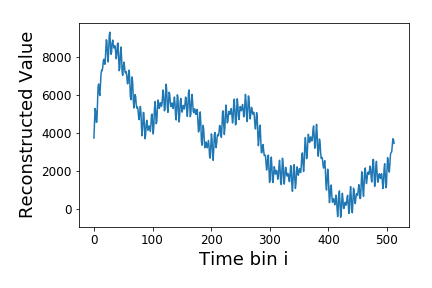
\includegraphics[width=\linewidth]{Reconstruction}
\caption{Reconstruction of the signal in figure \ref{fig:trend} using an inverse FFT. Note that the trend $g(i)$ does not appear as expected in the reconstruction. This result was one of many: each separate run of the program produced a different reconstruction based on the different random noise changes.}
\label{fig:Reconstruction}
\end{figure}

Next, a different method of uncovering the original $x(i)$ function was attempted. First, the $g(i)$ term was removed from $x(i)$. This new modified $x(i)$ was then Fourier transformed. The noise was again removed from the signal using only frequency magnitudes greater that $180$. It was found that using the suggested filtering value of 9 from the lab instructions did not yield the correct results. Using the filtered frequency spectrum, the inverse Fourier transform, that is the noiseless $x(i) - g(i)$ was obtained. Finally, the trend $g(i)$ was added back to the signal. Originally, this yielded a massive sinusoid without upward trend. To fix this, after the frequency spectrum was returned to the time domain, the result was re-normalized to the maximum of the original trend-less $x(i)$. This was cheating somewhat, as in real experiments, the maximum of the original function might not be known. Once the signal was re-normalized and had $g(i)$ added back in, the signal behaved more similarly to what was expected. Figure \ref{reconstruction_fixed} shows the final result.

\begin{figure}
\centering
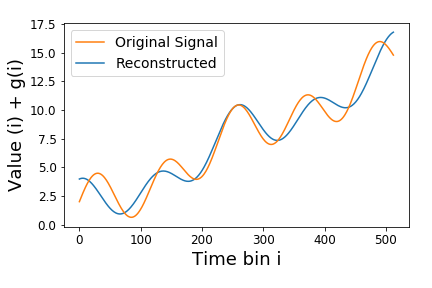
\includegraphics[width=\linewidth]{reconstruction_fixed}
\caption{Reconstruction of the original signal from figure \ref{fig:trend}. Note the aparent scale difference between the two lines.}
\label{fig:reconstruction_fixed}
\end{figure}

Trends have been shown to make Fourier analysis impossible without knowledge of the underlying trend. Even a slight trend in data could wreak havoc on the analysis. The trend in this example was shown to be stronger than the underlying frequencies, suggesting that different filtering regimes would be largely useless. This provides an effective encryption masking underlying periodicity. Unless the exact trend was known, the attempts to recover the original signal would be largely gibberish. By transmitting the trend function as some sort of key, this provides a basic form of encryption.

\subsubsection{Autocorrelation and Power Spectra}
The autocorrelation function and the power spectrum of signals are related. This may be demonstrated analytically with relative ease. Essential to these derivations is the Fourier shift theorem. The theorem provides a quick way to simply a Fourier transform when the function in question contains a shift in the coordinate being transformed. The theorem is derived below:
\begin{equation}
\begin{split}
\mathcal{F} \{f(t - a)\} = & \int_{-\infty}^{\infty} f(t-a) e^{2\pi i\omega t} dt \\
= & \int_{-\infty}^{\infty} f(t-a) e^{2\pi i\omega t} e^{2\pi i\omega a} e^{-2\pi i\omega a} dt \\
= & e^{2\pi i\omega a} \int_{-\infty}^{\infty} f(t-a) e^{2\pi i\omega t}  e^{-2\pi i\omega a} dt \\
= & e^{2\pi i\omega a} \int_{-\infty}^{\infty} f(t-a) e^{2\pi i\omega (t - a)} dt \\
= & e^{2\pi i\omega a} \int_{-\infty}^{\infty} f(t') e^{2\pi i\omega t'} dt' \\
= & e^{2\pi i\omega a} \mathcal{F} \{f(t)\}
\end{split}
\end{equation}

First, a proof will be shown for $C(\omega) = \sqrt{2\pi} Y^*(\omega)X^*(\omega)$:

\begin{equation}
\begin{split}
c(\tau) = & \int_{-\infty}^{\infty} y^*(t - \tau) x(t) dt\\
\mathcal{F} \{c(\tau)\} = & \mathcal{F} \{\int_{-\infty}^{\infty} y^*(t - \tau) x(t) dt\} \\
C(\omega) = & \int_{-\infty}^{\infty} \int_{-\infty}^{\infty} y^*(t - \tau) x(t) e^{2\pi i \omega \tau} dt d\tau \\
= & \int_{-\infty}^{\infty} \int_{-\infty}^{\infty} y^*(-\tau) x(t) e^{2\pi i \omega t} e^{2\pi i \omega \tau} dt d\tau \\
= & \int_{-\infty}^{\infty}y^*(\tau) e^{2\pi i \omega (-\tau)}  d\tau \int_{-\infty}^{\infty}  x(t)  e^{2\pi i \omega t} dt \\
= &\sqrt{2\pi} Y^*(\omega)X(\omega)
\end{split}
\end{equation}

Related to the correlation function is the autocorrelation function. The autocorrelation function may be defined as a convolution of a function with itself. From this term's Fourier material, it has been stated that a convolution in one space is a product in the corresponding Fourier space. From this, the relation between the autocorrelation and the power spectrum of a signal have been linked. This may be proved, as shown below:

\begin{equation}
\begin{split}
AC(\tau) = & \int_{-\infty}^{\infty} y^*(t) y(t + \tau) dt\\
\mathcal{F} \{AC(\tau)\} = & \mathcal{F} \{\int_{-\infty}^{\infty} y^*(t - \tau) y(t) dt\} \\
AC(\omega) = & \int_{-\infty}^{\infty} \int_{-\infty}^{\infty} y^*(t - \tau) y(t) e^{2\pi i \omega \tau} dt d\tau \\
= & \int_{-\infty}^{\infty} \int_{-\infty}^{\infty} y^*(-\tau) y(t) e^{2\pi i \omega t} e^{2\pi i \omega \tau} dt d\tau \\
= & \int_{-\infty}^{\infty}y^*(\tau) e^{2\pi i \omega (-\tau)}  d\tau \int_{-\infty}^{\infty}  y(t)  e^{2\pi i \omega t} dt \\
= &\sqrt{2\pi} Y^*(\omega)Y(\omega) \\
= & \sqrt{2\pi} |Y(\omega)|^2
\end{split}
\end{equation}

The auto-correlation function of white noise was explored earlier in this assignment. The findings of that computation may be verified analytically. Given that white noise should exist equally at all, infinite frequencies in the frequency domain, the autocorrelation may be determined by reverse Fourier transform. To begin, an assumption is made that the power of all frequencies is $S(f) = k$.
\begin{equation}
\begin{split}
S(f) =& k \\
AC(\tau) =& \mathcal{F}^{-1} \{ S(f) \} \\
AC(\tau) =& \sqrt{2\pi} \int_{-\infty}^{\infty} k e^{-2\pi i f \tau} df \\
AC(\tau) =& \sqrt{2\pi}k \int_{-\infty}^{\infty} e^{- i \omega \tau} \frac{d\omega}{2\pi} \\
AC(\tau) =& \frac{k}{\sqrt{2\pi}} \int_{-\infty}^{\infty} e^{- i \omega \tau} d\omega \\
AC(\tau) =& \frac{k}{\sqrt{2\pi}} \delta(\tau) \\
\end{split}
\end{equation}
\subsection{Applications}
\subsection{The Lorenz System}
The Lorenz system is a description of physical systems where a large number of variables are interrelated through differential equations. For this example, a system with three variables and three parameters will be considered. Equations \ref{difs} shows the system of equations in question.
\begin{equation} \label{difs}
	\begin{split}
		\frac{\partial x}{\partial t} =& \sigma (y - x) \\
		\frac{\partial y}{\partial t} =& rx - y - xz \\
		\frac{\partial y}{\partial t} =& xy - bz \\
	\end{split}
\end{equation}

The equation will reach an equilibrium in the case where all the partial derivatives are zero. The $x$, $y$, and $z$ equilibrium values may be found analytically:
\begin{equation} \label{equilibrium}
	\begin{split}
		0 = \sigma (y - x) \quad \to  & \quad x_{eq} = y_{eq}\\
		0 = xy - bz \quad \to & \quad y_{eq} = \sqrt{(bz_{eq})}\\
		0 = rx - y - xz \quad \to & \quad z_{eq} = r-1\\
		\therefore x_{eq} = y_{eq} =& \sqrt{b(r-1)}
	\end{split}
\end{equation}
This is only true if $x = y \neq 0$. Otherwise, the other equilibrium state is
when all positions are at zero: $x = y = z = 0$.

Numerical solutions to the Lorenz equations were calculated using the
fourth-order Runge-Kutta scheme (RK4). In the first batch of simulations run,
different initial conditions were used while keeping the other variables
constant, with $\sigma = 10, b = 8/3, r = 28$. The phase spaces from these
simulations are shown in figure \ref{fig:sims_init}.

\begin{figure}
	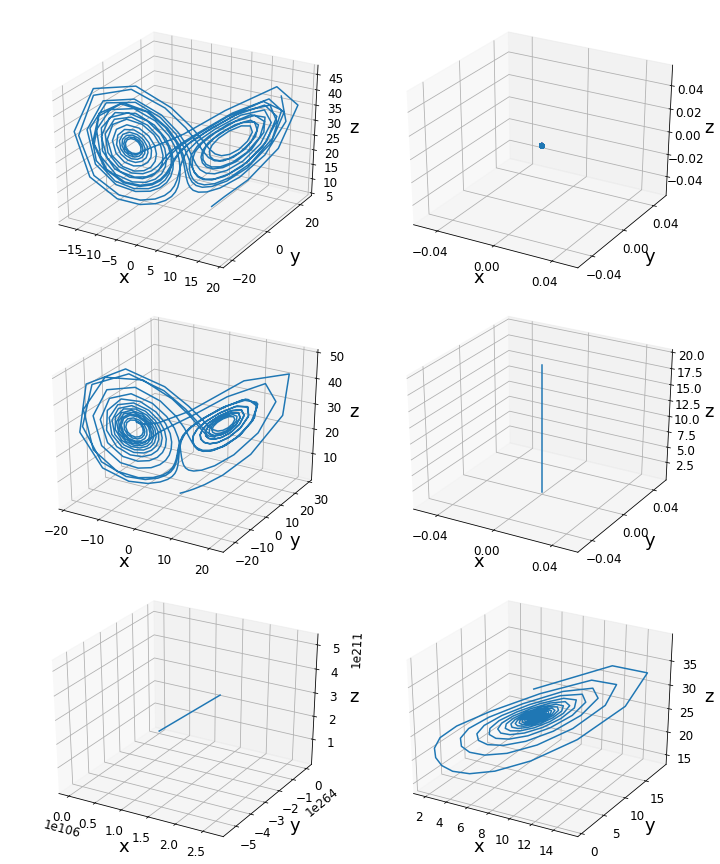
\includegraphics[width=\linewidth]{sims1.png}
	\caption{
		Simulations of the Lorenz system with varying initial conditions. The
		variables that remained constant are $\sigma=10, b=8/3, r=28$. Starting from
		the initial conditions are, from the top left,
		$(x_0, y_0, z_0) = \{
		(5, 5, 5),(0, 0, 0),
		(0.1, 0.1, 0.1), (0, 0, 20)$ $
		(100, 100, 100), (8.5,8.5, 27) \}$
	}
	\label{fig:sims_init}
\end{figure}

The top left panel begins with the initial condition $(x_0, y_0, z_0) = (5, 5,
5)$, and it is evident that one of the reasons that Lorenz may have used the
term ``butterfly'' to describe the evolution of this system because the solution
maps out two wings at an angle like a butterfly's. From the simulations, there
are four general ways the simulation can end up: orbiting in the butterfly
wings, circularly orbiting a single point, halting halfway between the two possible equilibrium points, or being ejected from the system in a straight line. When the system is plotted in the 'butterfly' case in an animation, the system never reaches equilibrium, instead orbiting around the points $(\pm 6\sqrt{2},\pm 6\sqrt{2}, 27)$. 

\begin{figure}
	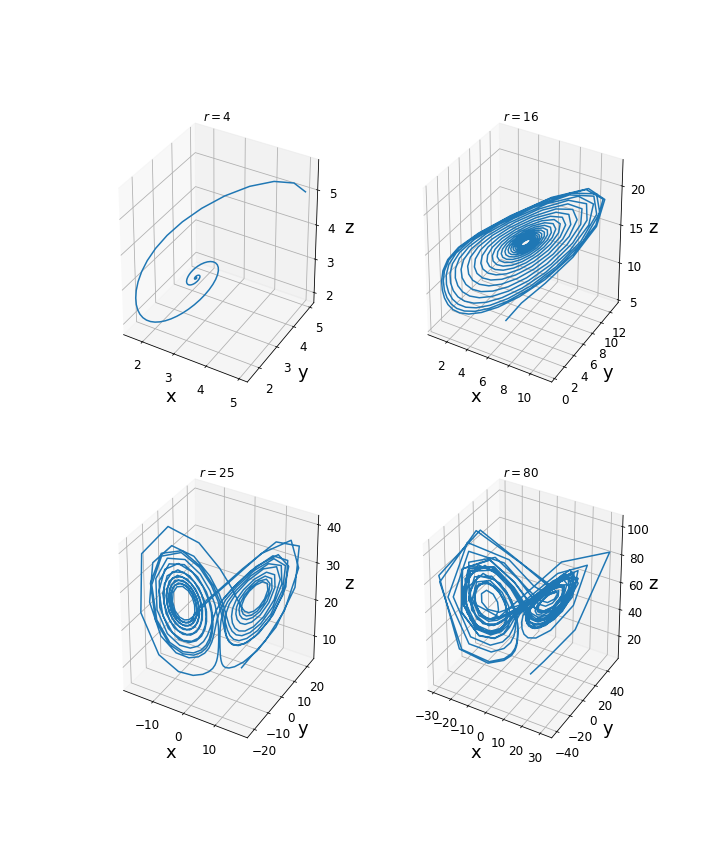
\includegraphics[width=\linewidth]{sims2.png}
	\caption{
		Simulations of the Lorenz system while varying the variable $r$. All other
		variables remain constant at $\sigma=10, b=8/3$ and initial condition $(x_0,
		y_0, z_0) = (5, 5, 5)$.
	}
	\label{fig:sims_vary_r}
\end{figure}

The second batch of simulations vary the value of $r$ and starting all of them
with the initial condition $(x_0, y_0, z_0) = (5, 5, 5)$, shown in figure
\ref{fig:sims_vary_r}. When the value is $0 < r < 24.74$, the system evolves as
a spiral, spiraling outwards faster as the value of $r$ decreases. In the other
regime, when $27.74 < r < 100$, system remains in orbit about the two butterfly
wings, with the steps increasing in size as the value of $r$ increases.

\begin{figure}
	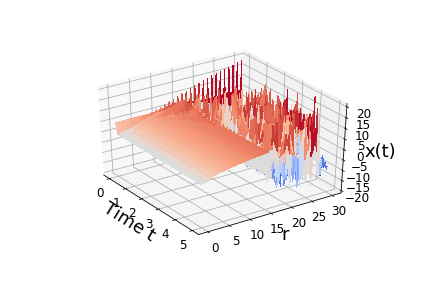
\includegraphics[width=\linewidth]{bifurcation.png}
	\caption{
		The bifurcation diagram of the Lorenz system obtained by gradually changing
		the value of $r$ from $0$ to $30$.
	}
	\label{fig:bifurcation}
\end{figure}

To further investigate the effect of $r$ on the system, the value was gradually
increased from $0$ to $30$ to create a bifurcation diagram of the Lorenz system,
shown in figure \ref{fig:bifurcation}. Once the value of $r$ was raised to the
value $27.74$, the system began to show pitchfork bifurcation, where the number
of fixed points transitions from one to three. At this critical point, the bifurcation plot becomes incredibly turbulent. In profile (i.e.: an r vs x(t) plot for given t) the r values begin to form sharp, close together peaks, resembling pitchforks.

The x component of the system was analyzed in a number of different ways. Figure \ref{fig:15spectra} shows the different Fourier power spectra for 5 different values of r. The DC component of the frequency was set to $0$ for each of the power spectra since the DC term tended to obscenely dominate. The power spectra show when periodic behaviour changes in the different r cases. When the system begins to orbit a single point, a single frequency appears in the power spectrum. After bifurcation begins, the power spectrum becomes far more messy, with periodic behaviour appearing at many more frequencies. The Fourier analysis was also extended to a three dimensional power spectrum shown in figure \ref{fig:power}. From this diagram it was apparent that much of the frequency data was clustered near the zero frequency, forming a ridge through the plot. This ridge seemed to split along certain r values. The system has near zero frequencies grow until approximately $r=14$, where a sudden decrease in these frequencies occurs. After this point, the spectra become more turbulent, splitting into the butterfly pattern, with the frequency spectrum broadening. Where earlier the identification of different patterns occured by fiddling with r on two dimensional plots, the three dimensional power spectrum provides a visual way to evaluate changes in the system. The Fourier analysis also describes the system well: low r regions are highly periodic (spiraling), and high r regions are much more chaotic. They are still periodic in some ways, but much more convoluted.

\begin{figure*}[p!]
\centering
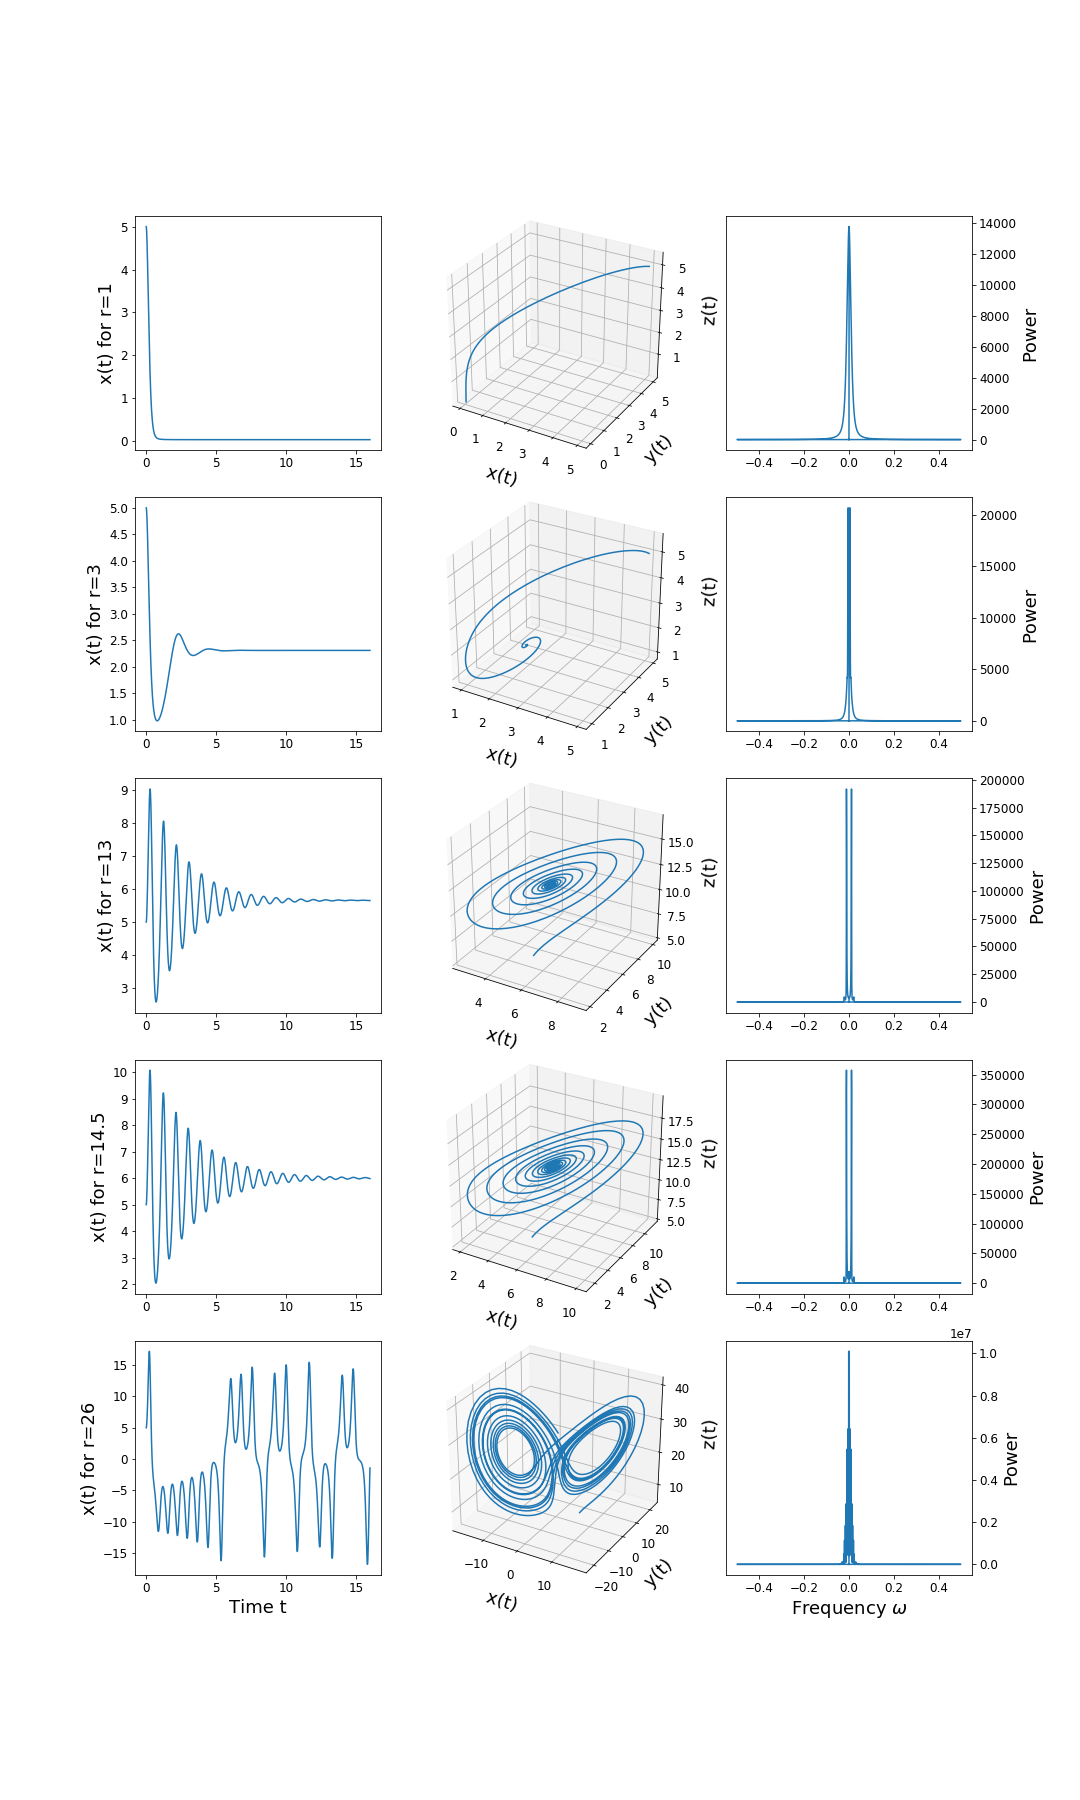
\includegraphics[trim= 0 +5cm 0 +12cm, width=\linewidth]{15spectra}
\caption{Fourier analysis of the Lorenz system for different r values. Each row represents a different value of r. The leftmost column shows the x position versus time for each r. The middle portion shows the trajectory through space, and the rightmost column the Fourier power spectrum.}
\label{fig:15spectra}
\end{figure*}

\begin{figure*}[t]
\centering
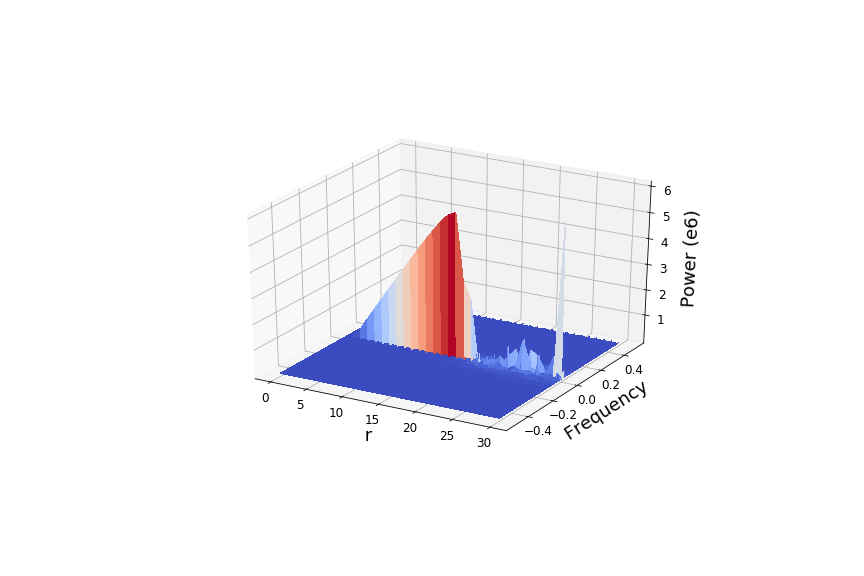
\includegraphics[width=\linewidth]{power}
\caption{3-dimensional power spectra for varying frequency and r.}
\label{fig:power}
\end{figure*}


\subsubsection{ODEs and the Fourier Transform}
The Fourier transform can be use to reduce the dimensionality of a differential equation. In essence, if the fourier transform is used, a PDE with two different differentials may be reduced to an ODE or and ODE to a polynomial equation. The original solution may then be recovered by reverse transforming the result. Below are a few examples of simplifying differential equations through Fourier transform:

\begin{equation}
\begin{split}
\mathcal{F} \{ m\ddot{x} + D\dot{x} + \kappa x &= n(t) \} \\
-\omega^2 \hat{x} +i\omega \hat{x} + \kappa\hat{x} &= \hat{n}(\omega)
\end{split}
\end{equation}

\begin{equation}
\begin{split}
\mathcal{F} \{ih \frac{\partial \psi}{\partial t} + \frac{h^2}{2m} \frac{\partial^2 \psi}{\partial x^2} &= 0 \} \\
-\omega h \hat{\psi} - \frac{ih^2}{2m} \frac{\partial^2 \hat{\psi}}{\partial x^2} = 0
\end{split}
\end{equation}

\begin{equation}
\begin{split}
\mathcal{F} \{ \frac{\partial^2 T}{\partial x^2} + \frac{\partial^2 T}{\partial z^2} &= \delta (x) \delta (z - a) \}\\
-k^2 \hat{T} + \frac{\partial^2 \hat{T}}{\partial z^2} &= e^{-2\pi ik x} \delta (z - a)
\end{split}
\end{equation}

\subsubsection{Heat Equation}
A common differential equation that is difficult to solve with non-complex analysis was the heat equation. The heat equation was defined as:
\begin{equation}
\begin{split}
\frac{\partial^2 T}{\partial x^2} &= -q(x)\\
q(x) =& \frac{\exp(-(x-x_0)^2/(2\sigma^2))}{\sqrt{2\pi\sigma^2}}
\end{split}
\end{equation}

This equation may be re-written using Fourier analysis. Two aids were used in this analysis: an integral table result for a zero-mean gaussian transform \cite{gauss_trans}, and the Fourier shift theorem to take care of the $x_0$ shift. Equations \ref{eq:gauss_transform} show this process.

\begin{equation}
\begin{split}
&\mathcal{F}\{ \frac{\partial^2 T}{\partial x^2} \} = \mathcal{F} \{ -q(x) \} \\
&-k^2 \hat{T} = -\hat{q}(x) \\
%&\\
%\hat{q}(x) =& \mathcal{F} \{ \frac{\exp(-(x-x_0)^2/(2\sigma^2))}{\sqrt{2\pi\sigma^2}} \} \\
%\hat{q}(x) =& e^{-2\pi ikx_0} \times \mathcal{F} \{ \frac{\exp(-(x^2/(2\sigma^2))}{\sqrt{2\pi\sigma^2}} \} \\
%\hat{q}(x) =& \exp\bigg( \frac{-\sigma^2 k^2}{2} - 2\pi ikx_0 \bigg) \\
%\hat{T} =& \frac{1}{k^2} \exp\bigg( \frac{-\sigma^2 k^2}{2} - 2\pi ikx_0 \bigg)
%
%\hat{q}(x) =& \frac{1}{\sqrt{2\pi\sigma^2}} \int_{-\infty}^{\infty} e^{2\pi ikx} e^{-(x-x_0)^2/\sqrt{2\sigma^2}} dx \\
%\hat{q}(x) =& \frac{1}{\sqrt{2\pi\sigma^2}} \int_{-\infty}^{\infty} \cos(2\pi kx) e^{-(x-x_0)^2/\sqrt{2\sigma^2}} dx \\
%\hat{q}(x) =& \frac{1}{\sqrt{2\pi\sigma^2}} e^{-2\pi ikx_0} \int_{-\infty}^{\infty} \cos(2\pi kx) e^{-x^2/\sqrt{2\sigma^2}} dx \\
%\hat{q}(x) =& \frac{1}{\sqrt{2\sigma^2}} e^{-2\pi ikx_0} \sqrt{\pi\sqrt{2\pi\sigma^2}} e^{-\pi^2 k^2 \sqrt{2\sigma^2}} \\
%\hat{T} &= \frac{e^{-\pi^2 k^2\sqrt{2\sigma^2} - 2\pi ikx_0/(2\sigma)^2}}{\sqrt{2k\pi\sigma^2}}
\end{split}
\label{eq:gauss_transform}
\end{equation}

In order to numerically solve the heat equation, the function $q(x)$ should be Fourier transformed to obtain $\hat{q}(k)$. This term may then be divided by $k^2$ and reverse transformed to obtain the original $T(x)$. This yields a problem in the case where $k=0$. Since python interprets a division by zero by returning 'nan', replacing this 'nan' with some DC term will allow the inverse transform to perform correctly. Figure \ref{fig:temp} shows the result of performing this method. Since the 'DC' term for $k=0$ has been replaced, this is not the exact answer, and instead is shifted by the non-existent DC term. It was therefore possible to shift this data so that all points had a non-negative temperature by shifting by the global minimum value. 

\begin{figure}
\centering
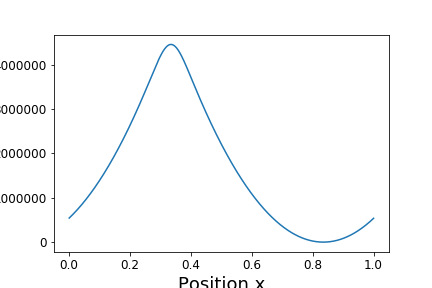
\includegraphics[width=\linewidth]{temp}
\caption{Temperature of a length $1$ rod corresponding to equation \ref{eq:gauss_transform}. The temperature may be off by a constant shift due to the deletion of the DC component in the frequency space.}
\label{fig:temp}
\end{figure}

The limits of Fourier transform solutions were considered using the function $q(x) = 0$. For this case, the familiar solution of $T(x) = Ax + B$ was obtained using analytical methods. For this particular case, the Fourier method of solutions breaks down. If we were to Fourier transform $q(x)$, the result would be $q(k)=0$. This in turn would lead to an overall solution $T(x) = 0$. This is a valid solution for the analysis above in the case $A=B=0$, however it is only one possible solution out of many. One way to consider this special case is that in its transformed form the Fourier inverse of temperature is $\hat{q}/k^2$. This acts to have a delta-esqe peak at zero frequency, except in the case where $\hat{q}=0$. To consider this from another direction, the fourier transform of the analytical solution was $\mathcal{F} = B\sqrt{(2\pi)}\delta (k) - iA\sqrt{(2\pi)}\delta(k)$ so the only information in Fourier space was contained at $k=0$, where the special case of $q=0$ removes the peaks.

\section{Discussion}
Different representations of the Fourier series can orovide different ways of looking at the same problem. While cosines and sines are useful for the initiate, the most common representation is the exponential representation. Section 2 above showed the connection between complex and sinusoidal coefficients. These relationships are related to the 'even' and 'uneven' aspects of a function in question. The $a$ coefficient represents the even part of a function, while the $b$ coefficients describe odd parts. This means that the $c$ coefficients are directly related to the $a$ and $b$ coefficients for even and odd functions, respectively. This can allow for a better intuition of results. An example of this was provided by a piecewise odd function. Since the function was odd, all of the $a$ terms vanished as may be seen in figure \ref{fig:Figure2}, where the $b$ terms survived.

Sampling windows and noise work to change a continuous source into the imperfect signal that many experiments rely upon. Where noise is extremely difficult to remove in the time domain, the frequency domain allows characterization of noise. In this experiment, the power spectra of different types of white noise were examined. White noise was characterized in the Frequency domain by an relatively uniform distribution of frequencies in theory. In actuality, the power spectra exhibited quite a bit of fluctuation around the expected mean of $S(\omega)=1$. This was likely due to three factors. First, the numpy random number generator used is known to be a poor random number generator. Secondly, all purely computational random number generators are actually pseudo-random, and will not exactly obey expectations. Lastly, the noise sample taken was somewhat limited in duration. As the noise sample length increases, the auto-correlation value will more closely approach zero beyond $k=0$ since for most numbers the denominator will grow faster than the numerator in the AC equation. 

Another method for examining noise was spectral subtraction. By transforming a signal into the frequency domain, the periodic signals will have well defined peaks compared to noise, which will allow data below a threshold to be removed, and the original signal to be recovered, with some error. This error is due to the impact of noise on a particular peak being difficult to evaluate. The experiments above showed that a signal must be significantly smaller than the amplitude of noise before it is well hidden. The above experiment found that the signal was still visible in the frequency domain until the noise was an order of magnitude larger than the signal. This is a relief for many in physics, as this means spectral isolation of signals can occur for even faint signals.

Trends were seen to be an effective way to mask the spectral signature of a signal. The peak caused by a trend tended to completely obscure underlying frequency data, and rendered spectral subtraction largely useless. If the equation of the trend is known, subtracting the trend from the original signal allowed underlying frequency data to be seen with some error. This suggests a rather simple method for encrypting data, which may be decrypted by a recipient with knowledge of the trend. An interesting test for a future experiment would be to test the effectiveness of least squares methods in effectively determining a trend. 

The Fourier transform was shown to be a technique to transform many differential equations into algebraic equations. Many simple differential equations were turned into quadratic equations which would be quickly solvable in one's head. While simple differential equations are made quite trivial with this method, they were already solvable with calculus methods. Where Fourier transforms really shine however, is with non-homogeneous differential equations. Non-homogeneous differential equations often required complicated methods to solve, and many were not solvable. If a function modifying a homogeneous equation was Fourier transformable, it had the possibility of being solved in the frequency domain, where the equation might be easier.

A transformed differential equation, specifically the heat equation, was examined. In this case, the boundary values made analytical solving of the transformation integral difficult. This was overcome by numerically evaluating a Gaussian function $q(x)$ on the interval $0 \leq x \leq 1$ and then using a fast Fourier transform to evaluate it. In the frequency domain, the $\hat{T}$ function could then be obtained by dividing by $k^2$. This however demonstrated a difficulty in using Fourier analysis to solve differential equations. When dividing by some variable, one must ensure that variable is not zero. Hence, an analytical solution was not possible for this differential equation, since it was possible for $k$ to equal zero. This is somewhat navigible however, as the $k=0$ term only yields a constant shift in the $x$ domain. As long as the system has some initial condition for $T$, the missing vertical shift should be recoverable.

\section{Conclusion}



\begin{thebibliography}{00}
	\bibitem{ouyed}
	Ouyed and Dobler, PHYS 581 course notes, Department of Physics and Astrophysics, University of Calgary (2016).
	\bibitem{NR}
	W. Press et al., \emph{Numerical Recipes} (Cambridge University Press, 2010) 2nd. Ed.
	\bibitem{Code}
	C. Hass and J. Burniston, MCMC Hill Climbing. Jupyter notebook, 2018.
	\bibitem{gauss_trans}
	K. Derpanis, Fourier Transform of the Gaussian, 2005, accessed at \url{http://www.cse.yorku.ca/~kosta/CompVis_Notes/fourier_transform_Gaussian.pdf}.
	\bibitem{RK4}
	Rosetta Code, "Runge-Kutta method", online publication: \url{https://rosettacode.org/wiki/Runge-Kutta_method.}
\end{thebibliography}

\section{Appendix}
For access to the source codes used in this project, please visit \url{https://github.com/Tsintsuntsini/PHYS_581} for a list of files and times of most recent update.
	
\end{document}